\documentclass[11pt]{article}

\usepackage[T1]{fontenc}
\usepackage[utf8]{inputenc}
\usepackage[ngerman]{babel}
\usepackage{amsmath, amssymb}
\usepackage{graphicx}
\usepackage{booktabs}
\usepackage[margin=2.5cm]{geometry}
\usepackage{csquotes}
\usepackage[hidelinks]{hyperref}

\graphicspath{{figures/}}

\newcommand{\nin}{n^{(i),\mathrm{in}}}
\newcommand{\nbar}{\overline{n}}

\title{Zellwachstum bei großer phänotypischer Heterogenität\\
\large Ein Finite-Volumen-Modell für konkurrierende Zellpopulationen}
\author{Joschik Brunow \and Jakob Krautmacher \and Lucas Posern}
\date{Wintersemester 2025/26}

\begin{document}
\maketitle

\begin{abstract}
\noindent
Wir simulieren das Wachstum von Gewebe, in dem sich mehrere Zelltypen zugleich
bewegen, vermehren und um Platz konkurrieren. Grundlage ist das Modell von
Dębiec, Mandal und Schmidtchen (2025): Alle Zellen folgen dem negativen
Gradienten eines gemeinsamen Drucks (Darcy-Gesetz) und wachsen logistisch, bis
das Gewebe lokal gefüllt ist. Wir leiten das Modell her, diskretisieren es mit
einem Finite-Volumen-Verfahren und zeigen Simulationen für $N$ Spezies in einer
Dimension sowie für zwei Spezies in zwei Dimensionen. In beiden Fällen trennen
sich anfangs gemischte Populationen im Zeitverlauf in räumlich getrennte
Bereiche.
\end{abstract}

\tableofcontents

\section{Einleitung}
In der Tumorforschung hilft es, die Entwicklung von Gewebe zu simulieren, um sie
vorherzusagen und besser zu verstehen. Wir stellen ein Modell vor, das
verschiedene Zelltypen mit unterschiedlichen Wachstumseigenschaften abbildet. Im
$d$-dimensionalen Raum lösen wir ein System partieller Differentialgleichungen,
dessen Lösung die Dichteverteilungen aller $N$ Phänotypen über die Zeit $t$
beschreibt.

Wir erklären zunächst das Modell. Anschließend stellen wir eine Implementierung
im eindimensionalen Raum für $N$ Spezies vor und zeigen danach Ergebnisse für
zwei Spezies im zweidimensionalen Raum. Beide Umsetzungen lösen das System mit
der Methode der finiten Volumen.

\section{Das mathematische Modell}
\label{sec:modell}
Wir erklären das Zellwachstumsmodell nach Dębiec, Mandal und Schmidtchen (2025).
Wir betrachten $N$ verschiedene Phänotypen und modellieren die Zeit kontinuierlich;
in der Implementierung diskretisieren wir sie anschließend. Die räumliche
Dimension $d \in \mathbb{N}$ halten wir allgemein.

\subsection{Zusammenhang von Druck und Geschwindigkeit}
Wir untersuchen zuerst, wie der Druck an verschiedenen Punkten die Bewegung, also
Geschwindigkeit und Richtung, beeinflusst. Wir gehen von einer Masse aus, die
überall dieselben Eigenschaften besitzt, bis auf den Druck $p \colon \mathbb{R}^d
\to \mathbb{R}$. Die Bewegung ist ein Vektorfeld $v \colon \mathbb{R}^d \to
\mathbb{R}^d$, das jedem Punkt Richtung und Geschwindigkeit $\lVert v \rVert$
zuordnet. Das Darcy-Gesetz verknüpft beide Größen:
\begin{equation}
    v(x) = -\nabla p(x).
\end{equation}
Der negative Gradient von $p$ zeigt in Richtung des steilsten Abstiegs und steht
orthogonal auf den Höhenlinien von $p$. Die Masse bewegt sich also vom höchsten
Druck zum niedrigsten, wie man es erwartet.

Dieses Modell bleibt vereinfacht. Es sagt nichts darüber aus, wie sich der Druck
in Zukunft verhält, da $v$ und $p$ nicht von der Zeit $t$ abhängen. Zusätzlich
nehmen wir eine Viskosität $\nu = 0$ an, sodass sich die Masse ohne Verzögerung
bewegt. Wir behalten diese Annahme bei, weil sie Gleichungen und Implementierung
deutlich vereinfacht.

\subsection{Das Modell für endlich viele Spezies}
\subsubsection{Bezeichnungen}
Sei $N \in \mathbb{N}$ die Anzahl der Spezies. Mit $n^{(i)}(x, t)$ bezeichnen wir
die Dichte der $i$-ten Spezies am Punkt $x \in \mathbb{R}^d$ zur Zeit $t \ge 0$
für jedes $i \in \{1, \dots, N\}$. Die durchschnittliche Dichte am Ort $x$ zur
Zeit $t$ ist
\begin{equation}
    \nbar(x, t) := \frac{1}{N} \sum_{i=1}^{N} n^{(i)}(x, t).
\end{equation}
Der Übersicht halber lassen wir die Argumente $(x, t)$ bei $n^{(i)}$ und $\nbar$
weg.

\subsubsection{Differentialgleichung}
Die Entwicklung der Dichten über die Zeit beschreibt für jeden Phänotyp $i \in
\{1, \dots, N\}$ die partielle Differentialgleichung
\begin{equation}
    \frac{\partial n^{(i)}}{\partial t}
    = \nabla \cdot \bigl( n^{(i)} \nabla \nbar \bigr) + n^{(i)} G^{(i)}(\nbar).
    \label{eq:pde}
\end{equation}
Der Nabla-Operator $\nabla = \bigl( \tfrac{\partial}{\partial x_1}, \dots,
\tfrac{\partial}{\partial x_d} \bigr)$ fasst die $d$ partiellen Ableitungen
zusammen. Der Term $\nabla \nbar$ beschreibt die Gesamtbewegung aller Zellen nach
dem Darcy-Gesetz. Multipliziert mit der Dichte $n^{(i)}$ ergibt sich die
tatsächliche Geschwindigkeit der jeweiligen Spezies, und die Divergenz $\nabla
\cdot (n^{(i)} \nabla \nbar)$ gibt an, wo die Dichte des Phänotyps zu- oder
abnimmt.

Entstehen und sterben keine Zellen, verschwindet der zweite Summand, und es
bleibt reiner Transport:
\begin{equation}
    \partial_t n^{(i)} = \nabla \cdot \bigl( n^{(i)} \nabla \nbar \bigr).
\end{equation}

\subsubsection{Die Wachstumsrate}
Der zweite Summand beschreibt über die Wachstumsfunktion $G^{(i)}$ das Verhalten
der Zelltypen. Wir definieren $G^{(i)}$ für jeden Phänotyp einzeln; sie hängt von
$i$ und von der durchschnittlichen Dichte $\nbar \in \mathbb{R}$ ab. Sei
$G^{(i)} \colon \mathbb{R}_+ \to \mathbb{R}$, $\nbar \mapsto G^{(i)}(\nbar)$ mit
folgenden Eigenschaften:
\begin{itemize}
    \item[(G1)] \emph{Stetige Differenzierbarkeit:} $G^{(i)} \in C^1(\mathbb{R})$.
    \item[(G2)] \emph{Strenge Monotonie:} $\exists\, \alpha > 0$ mit
    $\partial_{\nbar} G^{(i)}(\nbar) \le -\alpha$ für alle $\nbar \in \mathbb{R}$.
    \item[(G3)] \emph{Homöostatischer Druck:} für jedes $i$ existiert eine Dichte
    $n^{\star}_{(i)} > 0$ mit $G^{(i)}(n^{\star}_{(i)}) = 0$. Den größten dieser
    Werte nennen wir $\nbar^{\star} := \max_{i} n^{\star}_{(i)}$. Er hängt weder
    von $x$ noch von $t$ ab, sondern ist für jedes $i$ konstant.
\end{itemize}
Die strenge Monotonie (G2) bildet ab, dass sich Zellen umso schlechter teilen, je
höher der Druck um sie herum ist, weil dann weniger Platz für neues Gewebe bleibt.
Der homöostatische Druck (G3) ist der Punkt, an dem sich Sterbe- und
Vermehrungsrate ausgleichen. Aus $n^{\star} > 0$ folgt, dass jede Spezies bei
hinreichend kleiner Dichte positiv wächst, und die Monotonie sichert genau eine
Nullstelle. Negatives Wachstum wird also erst wieder positiv, sobald der Druck
genug nachgelassen hat.

Die Wachstumsrate erhält als Argument die durchschnittliche Dichte $\nbar$ und
wird mit der Dichte der Spezies an diesem Ort multipliziert. So entsteht die
absolute Wachstumszahl, die zur Bewegung im Raum addiert wird und in die zeitliche
Änderung der Dichteverteilung einfließt.

\subsubsection{Anfangsbedingung}
\label{sec:anfang}
Um den Prozess zu simulieren, brauchen wir eine Anfangsverteilung für jeden
Phänotyp. Sei $\nin \colon \mathbb{R}^d \to [0, \infty)$ die Anfangsverteilung mit
folgenden Eigenschaften:
\begin{itemize}
    \item[(I1)] \emph{$L^1$- und $L^\infty$-Integrierbarkeit:} $\nin \in
    L^1(\mathbb{R}^d) \cap L^\infty(\mathbb{R}^d)$.
    \item[(I2)] \emph{Beschränktheit:} $\nin(x) \le \nbar^{\star}$ (siehe (G3))
    für Lebesgue-fast alle $x \in \mathbb{R}^d$.
    \item[(I3)] \emph{Zentralität:} $\int_{\mathbb{R}^d} \nin(x)\, \lVert x
    \rVert^2 \, dx < \infty$.
\end{itemize}
Das Integral einer Dichte gibt die Gesamtzahl der Zellen des Typs an; über $L^1$
fordern wir daher endlich viele Zellen. $L^\infty$ beschränkt die Dichte auf jeder
Teilmenge mit positivem Lebesgue-Maß, was auch physikalisch sinnvoll ist. (I2)
verschärft das durch die obere Schranke $\nbar^{\star}$ aus (G3): mindestens ein
Phänotyp hat überall eine nicht-negative Wachstumsrate, das System startet also
nicht überbevölkert. (I3) gewichtet die Dichte mit $\lVert x \rVert^2$, sodass
Werte nahe dem Ursprung wenig, weit entfernte Werte stark zählen. Ist dieses
Integral endlich, halten sich die meisten Zellen anfangs zentral nahe dem Ursprung
auf und breiten sich im weiteren Verlauf nach Darcy-Gesetz aus.

Zusammen mit gegebenen $G^{(i)}$ und $\nin$ ergibt sich für alle $i \in \{1,
\dots, N\}$ das finale System
\begin{equation}
    \begin{aligned}
        \partial_t n^{(i)} &= \nabla \cdot \bigl( n^{(i)} \nabla \nbar \bigr)
        + n^{(i)} G^{(i)}(\nbar), \\
        n^{(i)}(x, 0) &= \nin(x).
    \end{aligned}
\end{equation}

\section{Numerische Umsetzung des 1D-$N$-Spezies-Modells}
\label{sec:1d}
Wir setzen das Darcy-Modell aus Abschnitt~\ref{sec:modell} für endlich viele
Spezies in einer Raumdimension um. Der Fokus liegt auf der Diskretisierung, den
Modellannahmen und der Interpretation der Ergebnisse.

\subsection{Beispiel zur Diskretisierung}
Zur Illustration betrachten wir den Fall $d = 1$ mit $N = 2$ Spezies auf $\Omega =
[0, 3]$, grob zerlegt in drei Kontrollvolumina der Breite $\Delta x = 1$:
\[
    C_1 = [0, 1], \quad C_2 = [1, 2], \quad C_3 = [2, 3].
\]
Als Anfangsdichten wählen wir die stückweise konstanten Zellmittelwerte
\[
    n^{(1)} = (0.8,\ 0.2,\ 0), \qquad n^{(2)} = (0,\ 0.4,\ 0.6),
\]
woraus die mittlere Dichte $\nbar_j = \tfrac{1}{2}\bigl(n^{(1)}_j + n^{(2)}_j\bigr)
= (0.4,\ 0.3,\ 0.3)$ folgt. In 1D ergibt sich das Geschwindigkeitsfeld aus $v =
-\partial_x \nbar$. Diskrete Differenzen an den Zellgrenzen liefern
\[
    v_{1 \to 2} \approx -(\nbar_2 - \nbar_1) = 0.1, \qquad v_{2 \to 3} \approx 0.
\]
Masse fließt also von $C_1$ nach $C_2$, während zwischen $C_2$ und $C_3$ kein
Transport stattfindet. Das zeigt den Druckausgleich von hoher zu niedriger
mittlerer Dichte.

Für das Wachstum wählen wir $G^{(1)}(\nbar) = 1 - \nbar$ und $G^{(2)}(\nbar) = 0.5
- \nbar$. Der lokale Reaktionsterm $n^{(i)}_j G^{(i)}(\nbar_j)$ lässt beide Spezies
dort wachsen, wo sie vorhanden sind, denn in allen Zellen gilt $\nbar_j < 1$ bzw.
$\nbar_j < 0.5$. Ist $n^{(i)}_j = 0$, entsteht keine neue Spezies. Die
Gesamtdynamik
\[
    \partial_t n^{(i)} = \partial_x\bigl( n^{(i)} \partial_x \nbar \bigr)
    + n^{(i)} G^{(i)}(\nbar)
\]
verschiebt vorhandene Masse entlang des Gradienten der Gesamtdichte und verstärkt
oder hemmt die lokale Dichte je nach Gesamtbelegung. Dieses Minimalbeispiel zeigt
die beiden zentralen Mechanismen: druckgetriebenen Transport von hoher zu
niedriger mittlerer Dichte, und Wachstum, das $\nbar$ lokal reguliert. Im nächsten
Schritt berücksichtigen wir beide Effekte pro Zeitschritt gemeinsam.

\subsection{Diskretisierung und Parameterwahl}
Das Gebiet ist das Intervall $[0, L]$, unterteilt in $J$ äquidistante
Kontrollvolumina der Breite $\Delta x = L / J$. Die Unbekannten sind die
Zelldichten $n^{i}_j(t) \approx n_i(x_j, t)$ der $N$ Spezies in den
Zellmittelpunkten $x_j$. Wir simulieren bis zur Endzeit $T$ mit fester
Schrittweite $\Delta t$. Den Druck wählen wir als
\begin{equation}
    p(\rho) = \rho^\gamma, \qquad \rho = \sum_{i=1}^{N} n_i,
\end{equation}
wobei $\gamma > 1$ einen stark anwachsenden Druck bei hohen Gesamtdichten
erzeugt. Die Spezies unterscheiden sich allein durch ihre konstanten
Wachstumsraten $r_i$. Dazu diskretisieren wir ein Intervall $[r_{\min},
r_{\max}]$ gleichmäßig, permutieren es zufällig und ordnen die Werte den Spezies
zu. So entstehen heterogene, aber zeitlich konstante Wachstumsbedingungen. Als
Anfangsdaten betrachten wir zwei Varianten, eine strikt getrennte Verteilung und
überlappende Gaußprofile mit über das Intervall verteilten Maxima. In beiden
Fällen skalieren wir so, dass $\rho(x, 0) \le 1$ für alle $x$ gilt und die
maximale Packungsdichte bereits zu Beginn erfüllt ist.

\subsection{Finite-Volumen-Schema}
\label{sec:fv1d}
Jede Spezies erfüllt
\begin{equation}
    \partial_t n_i + \partial_x (n_i v) = n_i r_i (1 - \rho), \qquad
    v = -\partial_x p(\rho).
\end{equation}
Wir diskretisieren diese Gleichung mit einem expliziten Finite-Volumen-Schema.
Es beruht auf der Bilanz über den Kontrollvolumina und erhält damit die
Gesamtmasse auf diskreter Ebene; eine ausführliche Darstellung geben Carrillo,
Chertock und Huang (2015). Aus den Dichten berechnen wir zunächst die Gesamtdichte
$\rho_j = \sum_i n^{i}_j$ und den Druck $p_j = (\rho_j)^\gamma$. Daraus folgt die
Geschwindigkeit an den Zellgrenzen über eine diskrete Ableitung,
\begin{equation}
    v_{j + \frac{1}{2}} = -\frac{p_{j+1} - p_j}{\Delta x},
\end{equation}
mit kein-Fluss-Randbedingungen $v_{1/2} = v_{J + 1/2} = 0$. Sobald die
Geschwindigkeit feststeht, diskretisieren wir den Transport mit einem
Upwind-Fluss, der den Dichtewert stromaufwärts nimmt:
\begin{equation}
    F_{i, j + \frac{1}{2}} =
    \begin{cases}
        v_{j + \frac{1}{2}}\, n^{i}_j,     & v_{j + \frac{1}{2}} \ge 0, \\[4pt]
        v_{j + \frac{1}{2}}\, n^{i}_{j+1}, & v_{j + \frac{1}{2}} < 0.
    \end{cases}
\end{equation}
Den Reaktionsterm setzen wir lokal als $R^{i}_j = n^{i}_j r_i (1 - \rho_j)$ an; er
liefert logistisches Wachstum mit Tragfähigkeit $\rho = 1$. Damit besteht ein
expliziter Zeitschritt aus vier Teilen: Druck und Geschwindigkeit, Flüsse,
Reaktionsterm und dem Update der Dichten. Negative Werte schneiden wir numerisch
ab. Eine hinreichend kleine Wahl von $\Delta t$ sichert die Stabilität.

\subsection{Modellannahmen}
\label{sec:annahmen1d}
Die 1D-Simulation beruht auf vier Annahmen: das Gewebe ist eindimensional; alle
Spezies erfahren dasselbe, von der Gesamtdichte abhängige Druckfeld; die lokale
Dichte ist durch $\rho \le 1$ beschränkt; und wir verwenden isolierende
Randbedingungen. Eine vollständige Übersicht aller Annahmen des Modells und beider
Implementierungen gibt Abschnitt~\ref{sec:overview}.

\subsection{Visualisierung und Phasentrennung}
Für ausgewählte Zeitpunkte zeigen wir zwei Darstellungen: die absolute Dichte
einer Spezies zusammen mit der Gesamtdichte, und den relativen Anteil einer
Spezies an der Gesamtpopulation.

\paragraph{Fall 1: strikt getrennte Anfangsverteilung.}
Zwei Spezies belegen zu Beginn disjunkte Bereiche, sodass Konkurrenz zunächst nur
an der Grenzfläche auftritt. Die Spezies mit höherer Wachstumsrate erzeugt lokal
mehr Druck und verdrängt die langsamere. Nach Erreichen der maximalen Gesamtdichte
stellt sich eine stabile, räumlich getrennte Konfiguration ein
(Abbildung~\ref{fig:fall1}).

\begin{figure}[htbp]
    \centering
    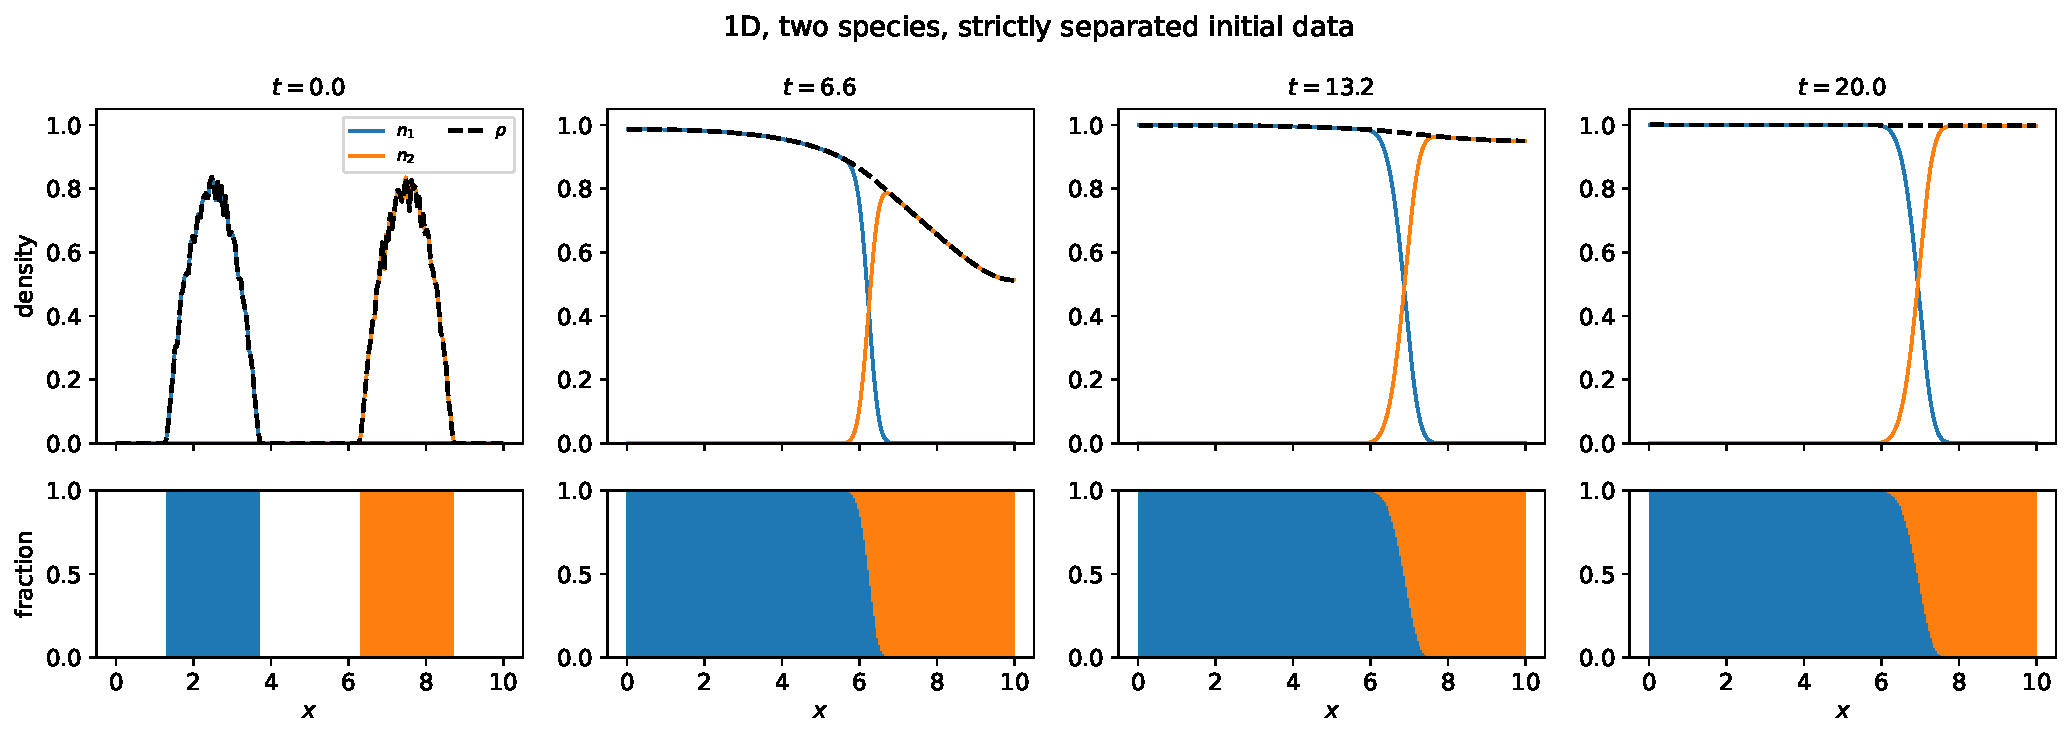
\includegraphics[width=\textwidth]{fig_1d_separated.pdf}
    \caption{Fall 1: Entwicklung der Zellverteilung bei strikt getrennter
    Anfangsverteilung.}
    \label{fig:fall1}
\end{figure}

\paragraph{Fall 2: überlappende Gaußprofile.}
Mehrere Spezies starten mit überlappenden Gaußprofilen und damit in direkter
Konkurrenz. In denselben Raumregionen bilden schneller wachsende Spezies höhere
Dichten und verdrängen langsamere. Im Zeitverlauf entsteht eine ausgeprägte
Phasentrennung in getrennte Domänen, während die Gesamtdichte die Schranke $\rho =
1$ erreicht (Abbildung~\ref{fig:fall2}).

\begin{figure}[htbp]
    \centering
    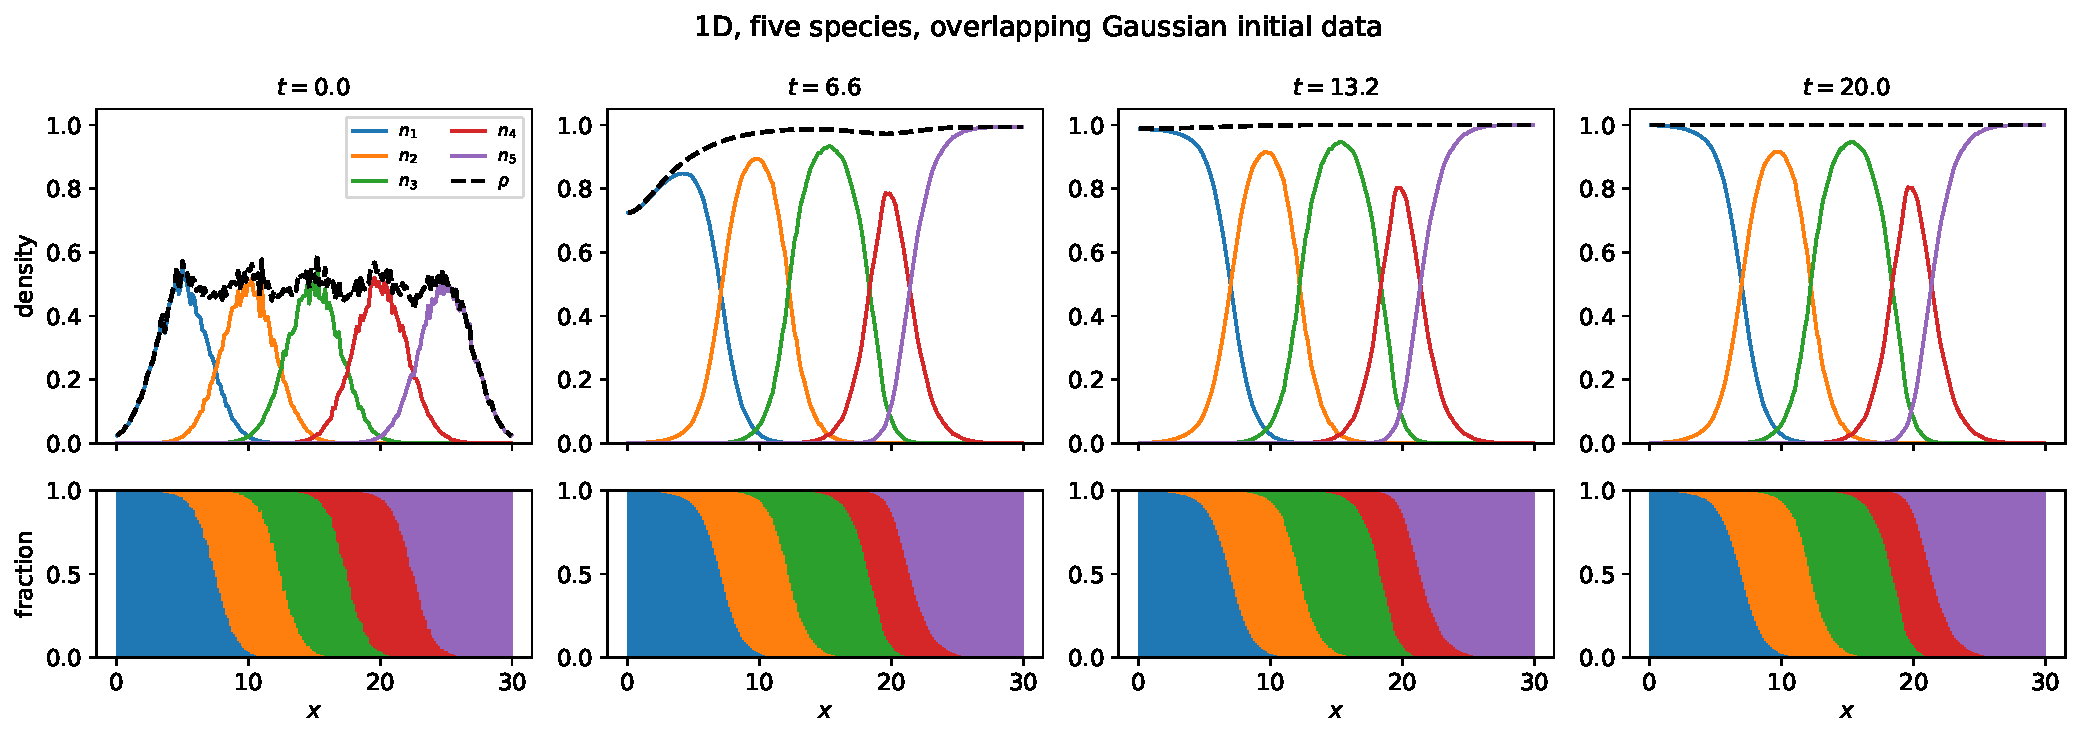
\includegraphics[width=\textwidth]{fig_1d_gaussian.pdf}
    \caption{Fall 2: Entwicklung der Zellverteilung bei überlappenden
    Gauß-Glocken.}
    \label{fig:fall2}
\end{figure}

\section{Numerische Umsetzung des 2D-2-Spezies-Modells}
\label{sec:2d}

\subsection{Aufbau und Parameter}
Wir implementieren die Simulation in Python als Klasse \texttt{TissueSim2D}. Alle
Attribute lassen sich verändern und alle Methoden flexibel aufrufen, was
Parameterstudien und Erweiterungen erleichtert. Die Klasse stellt folgende
Methoden bereit:
\begin{itemize}
    \item \texttt{\_\_init\_\_}: initialisiert Rechengitter, Modellparameter und
    Anfangsdichten.
    \item \texttt{update\_n}: berechnet aus den Dichten des vorherigen
    Zeitschritts die neuen Dichten mit Finite-Volumen-Schema und explizitem
    Euler-Verfahren.
    \item \texttt{run}: führt die Simulation über alle Zeitschritte aus und
    speichert regelmäßig Schnappschüsse.
    \item \texttt{visualize}: stellt beide Spezies, die Gesamtdichte und einen
    direkten Vergleich dar.
    \item \texttt{save} / \texttt{load}: sichern oder laden den vollständigen
    Simulationszustand.
\end{itemize}

Die wichtigsten Parameter sind die Gittergröße \texttt{grid\_size} (das Gitter
besteht aus \texttt{grid\_size} $\times$ \texttt{grid\_size} zellzentrierten
Kontrollvolumina), die Schrittzahl \texttt{count\_timesteps}, die Schrittweite
\texttt{dt}, das Speicherintervall \texttt{snapshot\_every} und der
Randbedingungstyp \texttt{boundary} (\texttt{neumann} oder \texttt{dirichlet}).
Das Verhalten der Spezies steuern die Wachstumsraten \texttt{G1}, \texttt{G2}, die
Konkurrenzkoeffizienten \texttt{comp1}, \texttt{comp2} (Wachstumshemmung durch die
jeweils andere Spezies), die Druckantwort \texttt{beta1}, \texttt{beta2} und die
Selbstdiffusion \texttt{eps1}, \texttt{eps2}. Die Anfangsverteilung legen
\texttt{center}, \texttt{peak}, \texttt{sigma} und \texttt{background} für beide
Spezies fest. Die Standardparameter sind symmetrisch, damit sich der Einfluss
einzelner Parameter isoliert untersuchen lässt.

\subsection{Finite-Volumen-Schema und Zeitdiskretisierung}
\subsubsection{Zu lösende Gleichungen}
Das Modell besteht aus zwei gekoppelten Erhaltungsgleichungen für $i, j \in \{1,
2\}$ mit $i \neq j$:
\begin{equation}
    \partial_t n_i + \nabla \cdot (n_i v_i) = \varepsilon_i \Delta n_i
    + G_i\, n_i (1 - n_i - c_i n_j), \qquad
    v_i = -\beta_i \nabla \nbar, \quad \nbar = \tfrac{1}{2}(n_1 + n_2).
\end{equation}
Gegenüber dem 1D-Modell kommen zwei Effekte hinzu: die Selbstdiffusion
$\varepsilon_i \Delta n_i$ und die asymmetrische Konkurrenz über die
Koeffizienten $c_i$.

\subsubsection{Räumliche Diskretisierung}
Die Dichten $n^{k,l}_i$ sind zellzentrierte Mittelwerte auf einem gleichmäßigen
Gitter mit $0 \le k, l \le N - 1$; die Flüsse werten wir an den Zellrändern $k \pm
\tfrac{1}{2}, l$ bzw. $k, l \pm \tfrac{1}{2}$ aus. Zuerst approximieren wir die
Geschwindigkeiten an den Rändern über finite Differenzen,
\begin{equation}
    v^{k + \frac{1}{2}, l}_{i, x} = -\beta_i \frac{n^{k+1, l} - n^{k, l}}{\Delta x},
    \qquad
    v^{k, l + \frac{1}{2}}_{i, y} = -\beta_i \frac{n^{k, l+1} - n^{k, l}}{\Delta y}.
\end{equation}
Daraus bilden wir den advektiven Fluss $F = v n$ mit stromaufwärts gewähltem
Dichtewert,
\begin{equation}
    F^{k + \frac{1}{2}, l}_x =
    \begin{cases}
        v^{k + \frac{1}{2}, l}_x\, n^{k, l},   & v_x \ge 0, \\[3pt]
        v^{k + \frac{1}{2}, l}_x\, n^{k+1, l}, & v_x < 0,
    \end{cases}
    \qquad
    F^{k, l + \frac{1}{2}}_y =
    \begin{cases}
        v^{k, l + \frac{1}{2}}_y\, n^{k, l},   & v_y \ge 0, \\[3pt]
        v^{k, l + \frac{1}{2}}_y\, n^{k, l+1}, & v_y < 0.
    \end{cases}
\end{equation}
Die Divergenz folgt aus der Differenz der Randflüsse,
\begin{equation}
    (\nabla \cdot F)^{k, l}
    = \frac{F^{k + \frac{1}{2}, l}_x - F^{k - \frac{1}{2}, l}_x}{\Delta x}
    + \frac{F^{k, l + \frac{1}{2}}_y - F^{k, l - \frac{1}{2}}_y}{\Delta y}.
\end{equation}
Der lokale Wachstumsterm lautet $R^{k, l}_i = G_i\, n^{k, l}_i \bigl(1 - n^{k, l}_i
- c_i n^{k, l}_j\bigr)$.

\subsubsection{Zeitdiskretisierung und Stabilität}
Nachdem Fluss-Divergenz und Reaktionsterm feststehen, integrieren wir mit einem
expliziten Euler-Schema:
\begin{equation}
    n^{k, l}_i(t + \Delta t) = n^{k, l}_i(t) + \Delta t \Bigl(
    -(\nabla \cdot F_i)^{k, l} + \varepsilon_i (\Delta n_i)^{k, l} + R^{k, l}_i
    \Bigr).
\end{equation}
Das explizite Verfahren unterliegt Stabilitätsschranken, einer CFL-Bedingung für
die Advektion und einer Diffusionsbedingung der Form $\Delta t \lesssim C \Delta
x^2 / \varepsilon_i$. Wir wählen $\Delta t$ empirisch so, dass die Lösungen für die
betrachteten Parameterbereiche stabil bleiben; eine formale Stabilitätsanalyse
führen wir nicht durch.

\subsubsection{Randbedingungen}
Wir behandeln den Rand auf zwei Arten. Die Neumann-Randbedingung setzt die
Randwerte durch konstante Extrapolation erster Ordnung aus dem Inneren fort;
dadurch verschwindet der Normalfluss und die Gesamtmasse bleibt erhalten. Die
Dirichlet-Randbedingung setzt alle Randzellen nach jedem Zeitschritt auf Null und
modelliert damit eine überlebensfeindliche Umgebung, in der Zellen am Rand sofort
entfernt werden.

\subsection{Visualisierung der Ergebnisse}
Die Visualisierung zeigt vier Heatmaps: die Dichte der ersten Spezies, die der
zweiten, die Gesamtdichte und einen direkten Vergleich beider. Ein Schieberegler
stellt den Zeitpunkt ein, eine Checkbox blendet die Konturen ein oder aus. Rot
steht für Spezies~1, Blau für Spezies~2.

\paragraph{Standardsimulation und Variationen.}
Ausgehend vom selben Anfangszustand ändern wir jeweils einzelne Parameter. Eine
erhöhte Wachstumsrate ($\texttt{G1} = 1.3$) lässt Spezies~1 sich schneller
ausbreiten und Spezies~2 verdrängen. Eine stärkere Druckantwort ($\texttt{beta1} =
3.0$) bewegt Spezies~1 deutlich schneller als Spezies~2. Ändert man mehrere
Parameter zugleich, lassen sich sehr verschiedene Zelltypen gegenüberstellen und
ihr Verhalten im Modell beobachten.

\begin{figure}[htbp]
    \centering
    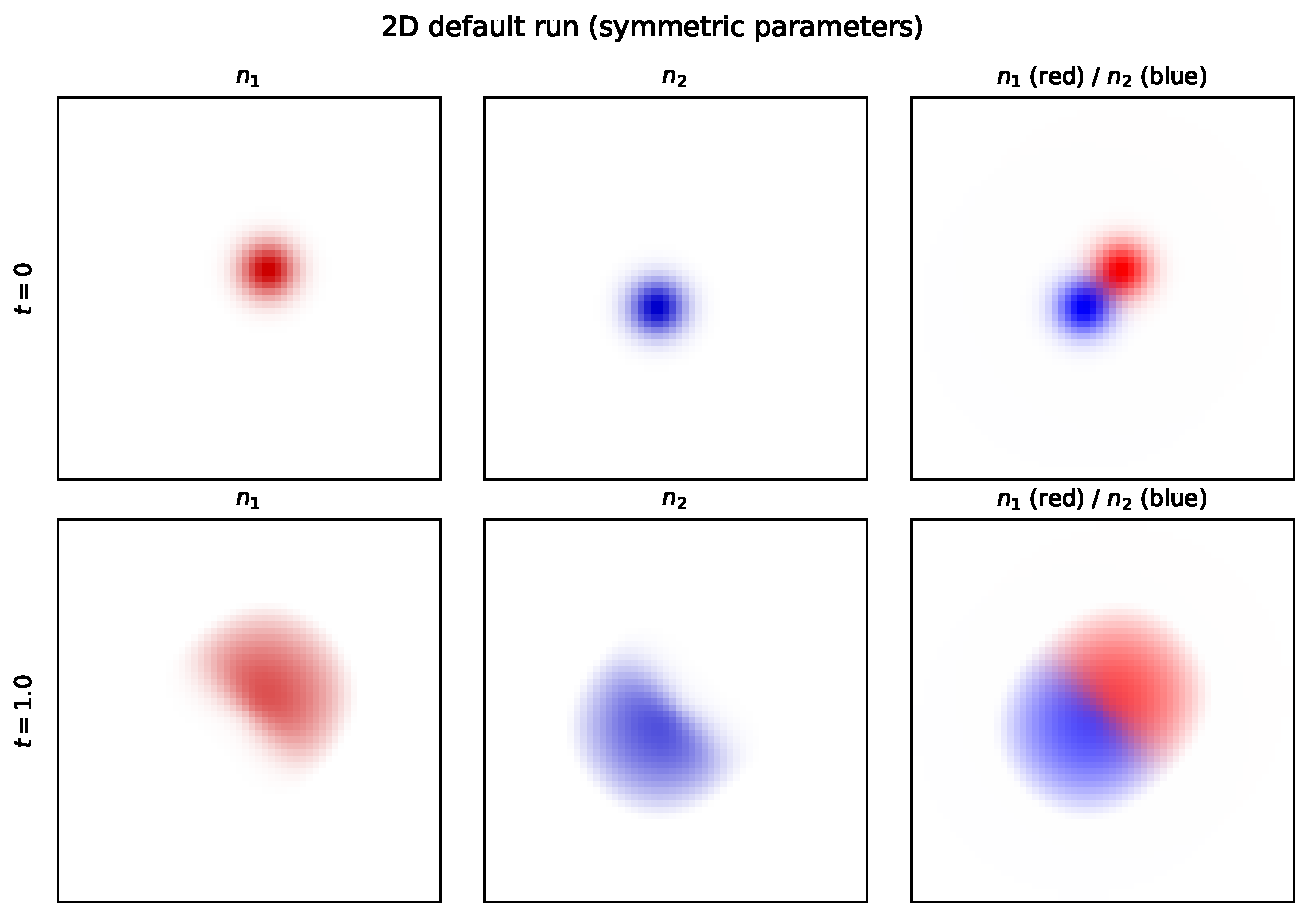
\includegraphics[width=\textwidth]{fig_2d_default.pdf}
    \caption{Standardsimulation mit symmetrischen Parametern: Anfangszustand und
    entwickelter Zustand. Rot steht für Spezies~1, Blau für Spezies~2.}
    \label{fig:2d_default}
\end{figure}

\begin{figure}[htbp]
    \centering
    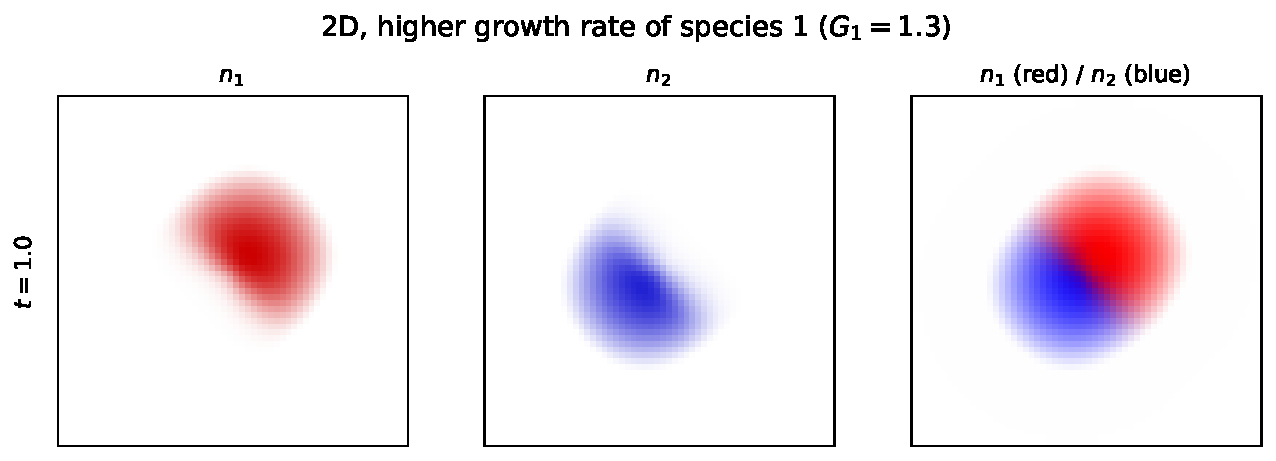
\includegraphics[width=0.92\textwidth]{fig_2d_growth.pdf}
    \caption{Höhere Wachstumsrate von Spezies~1 ($G_1 = 1.3$): Spezies~1 wächst
    schneller und verdrängt Spezies~2 etwas stärker.}
    \label{fig:2d_growth}
\end{figure}

\begin{figure}[htbp]
    \centering
    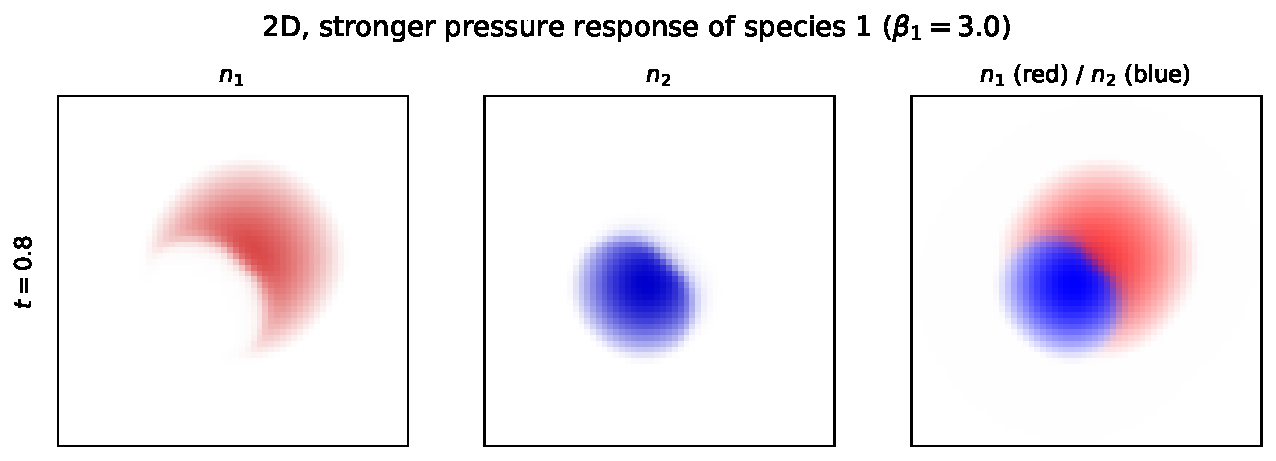
\includegraphics[width=0.92\textwidth]{fig_2d_pressure.pdf}
    \caption{Stärkere Druckantwort von Spezies~1 ($\beta_1 = 3.0$): Spezies~1
    fließt deutlich schneller auseinander als Spezies~2.}
    \label{fig:2d_pressure}
\end{figure}

\section{Übersicht aller Annahmen}
\label{sec:overview}
Tabelle~\ref{tab:annahmen} fasst die Annahmen zusammen, auf denen das Modell und
seine beiden Implementierungen beruhen.

\begin{table}[htbp]
    \centering
    \begin{tabular}{@{}p{4.2cm}p{10.3cm}@{}}
        \toprule
        \textbf{Bereich} & \textbf{Annahme} \\
        \midrule
        Bewegung (Darcy) & Geschwindigkeit $v = -\nabla p$; Viskosität $\nu = 0$,
        also Bewegung ohne Verzögerung. \\
        Druck & Gemeinsames Druckfeld $p(\rho) = \rho^\gamma$ mit $\gamma > 1$, das
        nur von der Gesamtdichte $\rho$ abhängt. \\
        Wachstum (G1--G3) & $G^{(i)} \in C^1$, streng monoton fallend
        ($\partial_{\nbar} G^{(i)} \le -\alpha$), mit genau einem homöostatischen
        Druck $n^{\star}_{(i)} > 0$. \\
        Anfangsdaten (I1--I3) & $\nin \in L^1 \cap L^\infty$, beschränkt durch
        $\nbar^{\star}$, mit endlichem zweiten Moment (zentrale Startverteilung). \\
        Sättigung & Maximale lokale Dichte $\rho \le 1$, bereits zu Beginn
        erfüllt. \\
        Geometrie & 1D-Modell auf $[0, L]$ bzw. 2D-Modell auf dem Einheitsquadrat. \\
        Rand & Isolierende (Neumann) Randbedingungen; im 2D-Fall alternativ
        Dirichlet. \\
        Zeit & Explizites Euler-Verfahren; $\Delta t$ empirisch unter der CFL- und
        Diffusionsschranke gewählt. \\
        2D-Zusatz & Selbstdiffusion $\varepsilon_i \Delta n_i$ und asymmetrische
        Konkurrenz $c_i$ zwischen den beiden Spezies. \\
        \bottomrule
    \end{tabular}
    \caption{Übersicht der Modell- und Implementierungsannahmen.}
    \label{tab:annahmen}
\end{table}

\begin{thebibliography}{9}
\bibitem{carrillo2015}
J.~A. Carrillo, A.~Chertock und Y.~Huang.
\newblock A finite-volume method for nonlinear nonlocal equations with a gradient
flow structure.
\newblock \emph{Communications in Computational Physics}, 17(1):233--258, 2015.

\bibitem{debiec2025}
T.~Dębiec, M.~Mandal und M.~Schmidtchen.
\newblock From finite to continuous phenotypes in (visco-)elastic tissue growth
models.
\newblock \emph{Journal of Differential Equations}, 437:113375, 2025.
\end{thebibliography}

\end{document}
